\chapter{Deep Learning}
\thispagestyle{fancy}
\label{chap:Deep Learning}
\noindent
Deep Learning ist ein Teilbereich des \ac{ML}. \ac{ML}-Algorithmen analysieren Daten automatisiert mittels mathematischer Methoden der Mustererkennung. \ac{DL}-Algorithmen bedienen sich hingegen vielschichtiger und hoch parametrisierter neuronaler Netze, um dem menschlichen Gehirn bestmöglich nachzuempfinden \cite[S.~455-457]{KHA19}. Dabei werden sehr große Datenmengen verarbeitet und analysiert, um einen Lerneffekt zu erzielen. Neben einer Eingabe- und einer Ausgabeschicht sorgen insbesondere die verborgenen Schichten für die prädizierte Tiefe. Hier werden Informationen weiterverarbeitet, abstrahiert und reduziert \cite[S.~131]{ZHA20}. Die potenziellen Einsatzmöglichkeiten gehen über die der \ac{ML}-Algorithmen hinaus. Der Aufbau neuronaler Netze sowie deren Funktionsweise und ausgewählte Architekturen werden in diesen Kapitel thematisiert. Hyperparameter und \ac{TL} schließen sich an.


\section{Neuronale Netze}
\noindent
Um den Aufbau und die Funktionsweise neuronaler Netze verstehen zu können, bedarf es zunächst der Beschreibung von Neuronen. Diese können im biologischen Sinne als Schalter verstanden werden, welche verschiedene Signale empfangen können und aktiviert werden, sobald genug Signale registriert wurden. Diese Aktivierung sendet folglich weitere Signale an andere Neuronen, wie \autoref{pic:ArtificialNeuron} im technischen Sinne exemplarisch skizziert \cite[S.~42]{KRI05}. Hierfür werden Aktivierungsfunktionen benötigt, welche die gewichteten Eingangssignale in ein Ausgangssignal konvertieren. Sie ermöglichen es, nicht-lineare Zusammenhänge zwischen den Eingangs- und den Ausgangsdaten herzustellen \cite[S.~134]{ZHA20}.\\

\begin{figure}[h!]
  \centering
  \fbox{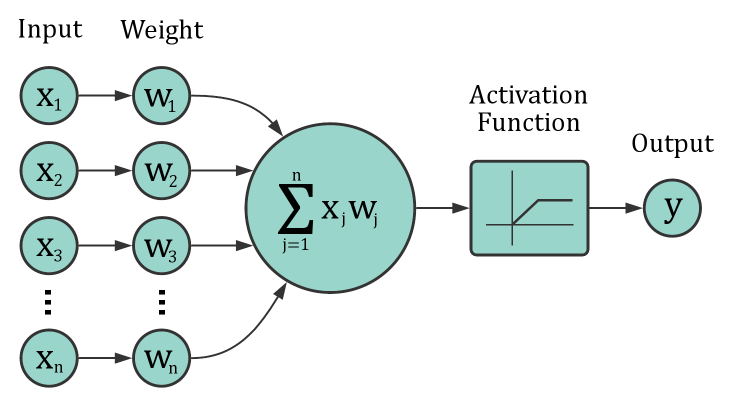
\includegraphics[width=0.6\linewidth]{./source/images/artificialneuron.png}}
  \caption{Aufbau eines künstlichen Neurons \cite{MCC20}.}
  \label{pic:ArtificialNeuron}
\end{figure}

\noindent
Die elementarste Form neuronaler Netze wird \ac{MLP} genannt. \ac{MLP} bestehen aus mehreren Schichten, deren Neuronen jeweils vollständig mit den Neuronen der umliegenden Schichten verbunden sind \cite[S.~131]{ZHA20}. Der Verständlichkeit halber veranschaulicht \autoref{pic:MultiLayerPerceptron} einen solchen Aufbau mit nur einer verborgenen Schicht, welche aus fünf Neuronen besteht.

\begin{figure}[h!]
  \centering
  \fbox{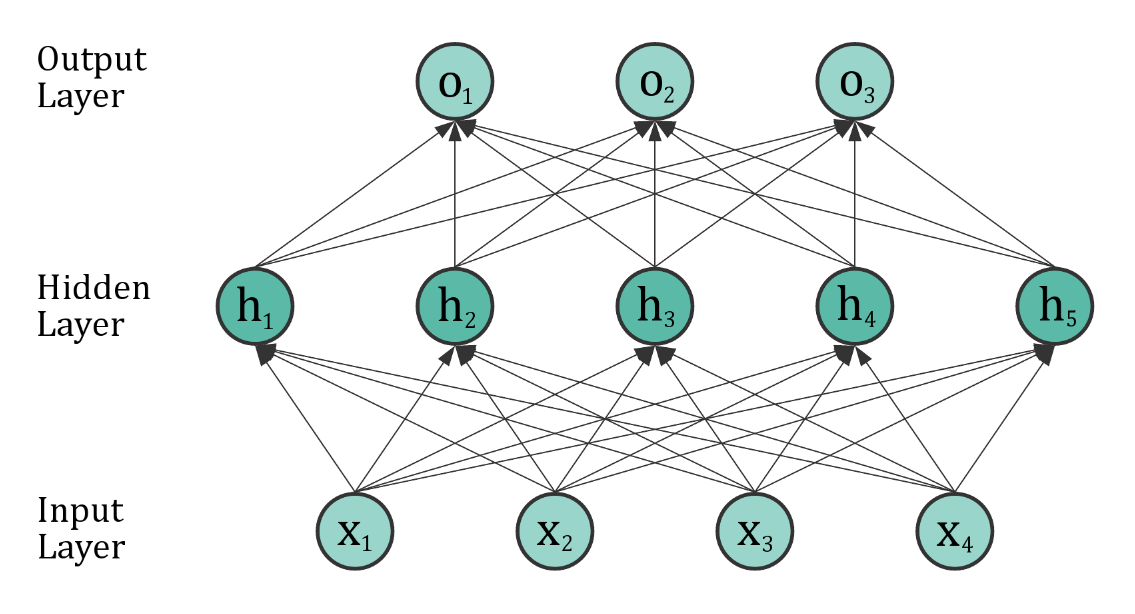
\includegraphics[width=0.6\linewidth]{./source/images/multilayerperceptron.png}}
  \caption{Aufbau eines MLP \cite[S.~133]{ZHA20}.}
  \label{pic:MultiLayerPerceptron}
\end{figure}

\noindent
Ziel der hoch parametrisierten neuronalen Netze ist es, komplexe Funktionen hohen Grades bestmöglich zu approximieren und so verschiedenste Probleme zu lösen. Der anvisierte Lerneffekt wird mithilfe des sogenannten Backpropagation-Algorithmus erreicht. Hierbei werden Eingangsdaten zunächst vorwärts durch ein neuronales Netz hindurch propagiert. Mithilfe einer Fehlerfunktion wird sodann die erwartete mit der tatsächlichen Ausgabe verglichen und bewertet. Über das Gradientenverfahren werden die Fehler nun rückwärts durch das neuronale Netz propagiert und somit die Gewichte in den Neuronen angepasst, insbesondere in den verborgenen Schichten. Ziel ist die Minimierung der Fehlerfunktion und letztlich die Optimierung der durch das neuronale Netz approximierten Funktion \cite[S.~140, 169]{ZHA20}.\\

\noindent
Der Trainingsprozess erfolgt optimalerweise über mehrere sogenannte Epochen. Hier werden dem neuronalen Netz verschiedene Eingangsdaten zugeführt und beidseitige Propagationen ausgeführt. Wichtig ist dennoch, kein Overfitting beziehungsweise Underfitting zu erzeugen. Dies würde bedeuten, dass das trainierte Modell zu sehr beziehungsweise zu wenig auf die Trainingsdaten angepasst ist. Ziel ist ein möglichst hoher Generalisierungseffekt des Modells, wie \autoref{pic:FittingTypes} zeigt. Das Modell sollte den Lernfortschritt auf noch unbekannte Daten adaptieren können und darauf eine hohe Genauigkeit erreichen. Es gibt verschiedene Ansätze, um beispielsweise Overfitting vorzubeugen. Hier seien insbesondere Batch Normalization, Dropout und Early Stopping genannt, wobei entsprechende Mechanismen an anderweitiger Stelle erläutert werden \cite[S.~143-149]{ZHA20}.

\begin{figure}[h!]
  \centering
  \fbox{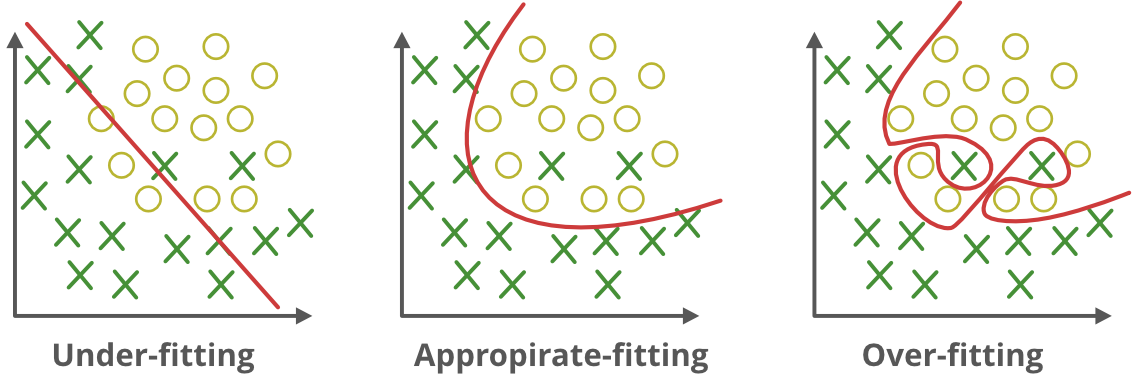
\includegraphics[width=0.65\linewidth]{./source/images/fittingtypes.png}}
  \caption{Typen von Generalisierungseffekten \cite{EDPOJ}.}
  \label{pic:FittingTypes}
\end{figure}


\section{Architekturen}
\noindent
Um mithilfe neuronaler Netze die \ac{ATS} zu modellieren, werden nun ausgewählte Architekturen vorgestellt. Diese gehen weit über die als Grundlage beschriebenen \ac{MLP} hinaus und verdeutlichen die Varietät neuronaler Netze. 


\subsection{Recurrent Neural Networks}
\noindent
\cite{ZHA20} ab Seite 361, 354, sequenzielle Daten fokussieren


\subsection{Encoder-Decoder Networks}
\noindent
\cite{ZHA20} ab Seite 377, 375, YAN19 S. 3 links unten und rechts unten, siehe außerdem \url{https://colab.research.google.com/drive/1WIk2bxglElfZewOHboPFNj8H44_VAyKE?usp=sharing#scrollTo=Gw3IZYrfKl4Z} für Encoder-Decoder-Rechtfertigung im entsprechenden Theorie-Teil, Skizzen von dort nutzen


\subsection{Attention in Neural Networks}
\noindent
\cite{ZHA20} ab Seite 389, 394 mit Self-Attention, Multi-Head-Attention, \cite{VAS17} nutzen, um Attention wissenschaftlich zu beschreiben, notfalls NLP für DL abhandeln, falls Inhalte hier erforderlich sind, dann entsprechend die Einleitungstexte anpassen


\subsection{Transformer Networks}
\noindent
\cite{ZHA20} ab Seite 398 mit MH-Attention, Encoder, Decoder, Training etc. + Transformer-based Encoder-Decoder-Models erwähnen, schon mal \cite{ROT20} bzgl. der Möglichkeit von Ersetzen des Encoder und und des Decoder durch vortrainierte multilinguale Modelle erwähnen, ebenfalls geeignet für sequenzielle Daten, Grenzen im nachfolgenden Kapitel bzgl. Transfer Learning genauer offenlegen, an \cite{RAF20} orientieren, ggf. \url{https://arxiv.org/pdf/1912.08777.pdf} referenzieren, oder auch \url{https://arxiv.org/pdf/2007.14062.pdf}


\section{Hyperparameter}
\noindent
Hyperparameter sind Parameter einer Architektur, die bereits vor dem eigentlichen Trainingsprozess definiert werden. Sie bedürfen einer separaten Optimierung, da sie eben dieses Training und folglich auch die Qualität des entstehenden Modells enorm beeinflussen. Ziel ist es hierbei, die beste Kombination aller Hyperparameter zu finden, um weiterhin die Fehlerfunktion zu minimieren \cite[S.~1]{YAN20}. Im weiteren Verlauf werden ausgewählte Hyperparameter peripher vorgestellt.\\


\subsection{Learning Rate}
\noindent
Die \ac{LR} ist ein Hyperparameter, der bestimmt, wie viel Einfluss jede einzelne Epoche im Trainingsprozess auf die Anpassung der Gewichte nimmt. Sie gilt mithin als wichtigster Hyperparameter einer Architektur \cite[S.~428]{ZHA20}.\\

\noindent
Dabei ist zunächst das Gradientenverfahren offenzulegen. Dieses dient der methodischen Lösung von Optimierungsproblemen. Entlang des negativen Gradienten wird das globale Minimum einer entsprechenden Fehlerfunktion gesucht, bis keine numerische Verbesserung mehr zu verzeichnen ist.\\

\noindent
Eine zu niedrige \ac{LR} kann den Trainingsprozess entweder stark verlangsamen oder dafür sorgen, dass kein Lernfortschritt mehr erzielt wird, da lokale Minima der Fehlerfunktion nicht übersprungen werden können und fälschlicherweise als globales Minimum interpretiert werden. Eine zu hohe \ac{LR} kann hingegen sehr abrupte Anpassungen der Gewichte verursachen, sodass potenziell auch das globale Minimum übersprungen werden kann \cite[S.~414-415]{ZHA20}. \autoref{pic:GradientDescent} verdeutlicht diese Bedingungen. Ziel ist allgemein eine möglichst schnelle Konvergenz.

\begin{figure}[h!]
  \centering
  \fbox{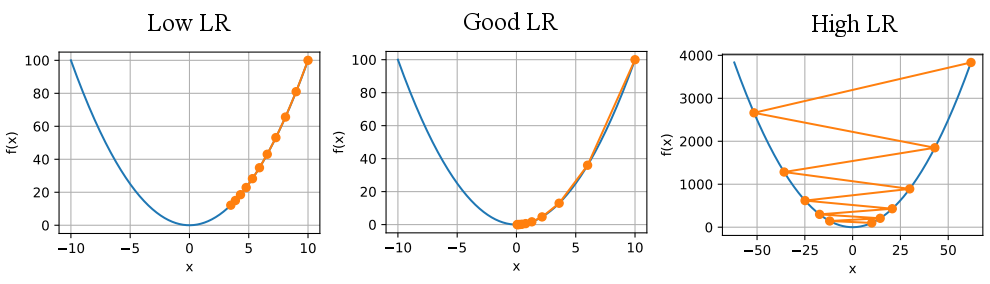
\includegraphics[width=0.7\linewidth]{./source/images/gradientdescent.png}}
  \caption{Konvergenz und Divergenz im Gradientenverfahren \cite[S.~429-430]{ZHA20}.}
  \label{pic:GradientDescent}
\end{figure}

\noindent
Neben der sorgfältigen manuellen Auswahl der \ac{LR}, etwa mithilfe eines sogenannten \ac{LR}-Schedule, ist es weiterhin möglich, eine adaptive \ac{LR} einzuführen. Hierbei wird die \ac{LR} in jeder Epoche verändert. Üblich ist hier die Reduktion der \ac{LR}, wenn bereits akzeptable Ergebnisse erreicht wurden \cite[S.~433]{ZHA20}. Außerdem existiert das stochastische Gradientenverfahren, welches pro Epoche nur eine Stichprobe der verfügbaren Trainingsdaten berücksichtigt. Hier ist von einem generalisierenden Effekt auszugehen \cite[S.~437]{ZHA20}.


\subsection{Momentum}
\noindent
Das Momentum unterstützt die bereits beschriebene \ac{LR} auf der Suche nach dem globalen Minimum in der Fehlerfunktion. Dabei berücksichtigt es den Durchschnitt vorheriger Gradienten. Auf dieser Grundlage wird entstiegen, in welche Richtung das stochastische Gradientenverfahren weiter absteigen soll, wie \autoref{pic:MomentumUpdate} zeigt. Das Momentum ist somit potenziell in der Lage, lokale Minima zu überspringen und die Suche erst im tatsächlichen globalen Minimum zu beenden \cite[S.~453-456]{ZHA20}.

\begin{figure}[h!]
  \centering
  \fbox{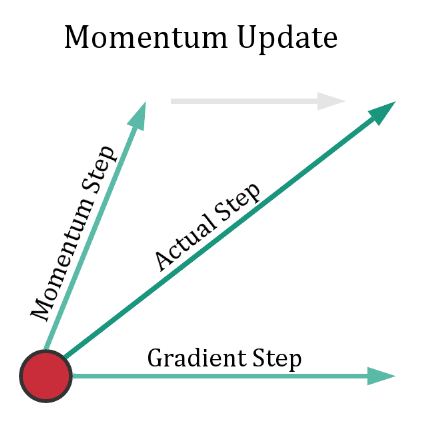
\includegraphics[width=0.35\linewidth]{./source/images/momentumupdate.png}}
  \caption{Gradientenverfahren unter Einfluss eines Momentums \cite{CSNOJ}.}
  \label{pic:MomentumUpdate}
\end{figure}

\noindent
Bei der Auswahl eines hohen Momentums sollte die \ac{LR} eher niedriger sein, oder anders herum. Eine Möglichkeit der stochastischen Optimierung ist hierbei \ac{ADAM}. Dieser Algorithmus übernimmt nicht nur die Auswahl der adaptiven \ac{LR}, sondern auch die Auswahl des entsprechenden Momentums. \ac{ADAM} arbeitet somit effizient für daten- und parameterintensive Probleme. Dabei konvergiert der Algorithmus üblicherweise schneller als vergleichbare Optimierungsalgorithmen \cite[S.~1-2]{KIN17}.


\subsection{Weight Decay}
\noindent
Weight Decay meint die Multiplikation der Gewichte einer Architektur nach jeder Epoche mit einem Faktor kleiner als eins, um sehr große Gewichte zu verhindern. Die Gefahr von Overfitting wird hierbei verringert, während sich die Generalisierung des Modells verbessert \cite[S.~154]{ZHA20}.


\subsection{Batch Size}
\noindent
Die Batch Size definiert die Größe der Stichprobe, welche je Epoche durch eine Architektur propagiert wird, ehe die entsprechenden Gewichte der Neuronen angepasst werden. Die Einführung einer Batch Size reduziert insbesondere den Rechenaufwand und den Speicherbedarf des Trainingsprozeses \cite[S.~446]{ZHA20}. Grundsätzlich lässt sich die optimale Kombination aller Hyperparameter durch Techniken wie Grid Search annähern \cite[S.~24]{YAN20}.


\section{Transfer Learning}
\noindent
\ac{TL} ist in den letzten Jahren wissenschaftlich immer bedeutsamer geworden, da \ac{DL}-Modelle heutzutage sehr komplex und Trainingsprozesse sehr zeit- und rechenintensiv sind. Unter \ac{TL} versteht man das Wiederverwenden bereits vortrainierter neuronaler Netze für die Lösung neuartiger Probleme. Das initiale Training obliegt hierbei meist großen Unternehmen oder Institutionen. Dabei werden die erprobten Modelle sodann als Startpunkt genutzt und nur noch auf die neuen Probleme adaptiert, anstatt eigene Modelle von Grund auf neu zu trainieren. Anwender profitieren hier zeitlich, qualitativ und technisch. Zumeist sind architektonische Anpassungen in den hinteren Schichten der vortrainierten Modelle erforderlich, sodass sie sich für die Lösung der neuen Probleme eignen, wie \autoref{pic:FineTuning} veranschaulicht. Zudem ist ein gezieltes weitergehendes Training mit entsprechenden Daten notwendig. Inwieweit die neuen Daten auf die vortrainierten Modelle einwirken sollen, ist individuell zu erproben \cite[S.~554]{ZHA20}.

\begin{figure}[h]
  \centering
  \fbox{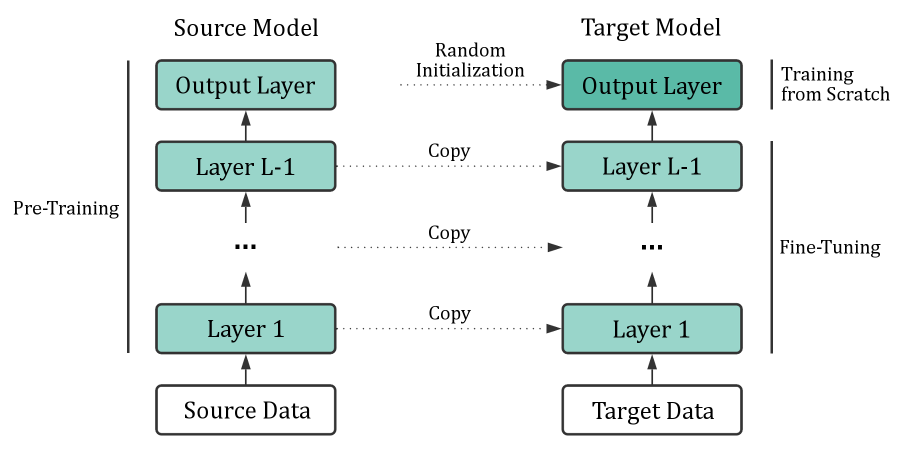
\includegraphics[width=0.6\linewidth]{./source/images/finetuning.png}}
  \caption{Fine-Tuning vortrainierter Modelle \cite[S.~555]{ZHA20}.}
  \label{pic:FineTuning}
\end{figure}

\noindent
\ac{TL} wird auch in dieser Arbeit genutzt. Einige Komponenten der bereits vorgestellten Architekturen, wie beispielsweise der Encoder oder auch der Decoder, können durch vortrainierte Modelle repräsentiert werden. Hier wird inhaltlich sowie kontextuell in den folgenden Kapiteln angeknüpft, da zunächst die Einführung weiterer \ac{NLP}-Grundlagen erforderlich ist. Die angeführten Vorteile von \ac{TL} können nichtsdestotrotz folgendermaßen zusammengefasst werden:

\begin{itemize}
	\item Zeitersparnis durch Überspringen des initialen Trainings
	\item Qualitätsanstieg und Generalisierung durch Berücksichtigung massenhafter Daten
	\item Reduktion von hardwaretechnischen Anforderungen, entsprechenden Kosten und dem Stromverbrauch
\end{itemize}
